The concept of implementation can be divided into the used packages (\emph{Stable Baselines3, Gym Pybullet Drones, ...}), the scripts, the environment classes and different support classes (\cref{fig:concept}).\\
Stable Baselines3 is used as implementation of the PPO algorithm (\cref{alg:ppo}) and SAC algorithm (\cref{alg:sac}) in order to achieve the tasks. Gym Pybullet Drones has already some environments and is the foundation of the simulation. It already provides a suitable step function and a well designed physics engine.\\
The scripts (\cref{sec:scripts}, lila) are used to either learn the agent on a given environment or evaluate it.\\
The environment classes(\cref{sec:env}, green) inherit from a \emph{Gym Environment} and models a MDP. By modelling this MDP precisely, it is defined what is learned later by the intelligent agent. It uses the wind class in order to model a harsh environment.
In addition, there are a couple of evaluation tools (\cref{sec:tools}, red), that supports the implemented classes.\\
\newline
The whole concept is implemented in Python3.x with the use of a \emph{conda environment}.

\begin{figure}[htp]
	\centering
	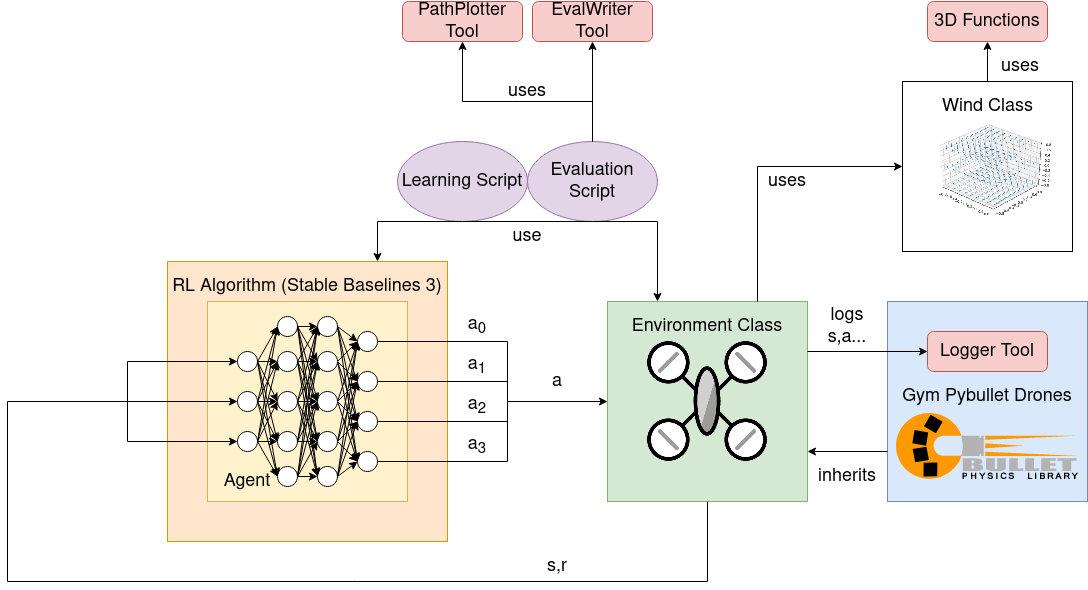
\includegraphics[width= \linewidth]{figures/concept.png}
	\caption{Concept of the implemented software: the different tools(red), scripts(violet) that are used in order to learn the intelligent Agent robust flight control with the use of RL.}
	\label{fig:concept}
\end{figure}
\newpage

\section{WindSingleAgentAviary Environment Class} \label{sec:env}
The \emph{WindSingleAgentAviary Class} is an implemntation of the environment that models the defined RL problem. It is highly adaptable and has the ability to model a range of MDPs with different action spaces and non-deterministic transitions caused by a random wind field (\cref{sec:wind}). 
Independently of this, the class still always models a goal environment, although the goal might be randomly sampled within a defined space (\cref{alg:sample}). 
These flexible parameters are summed up in different operating modes (\cref{sec:modes}). Nevertheless, this environement class only models learning to hover in goals. Theoretically, it is compatible with every RL algorithm that allows continous action spaces.
On initialization different parameters can be parsed to the environment class.

\begin{longtable}{|c|c|c|c|c|}
	\caption{Overview of the initialization parameters of the WindSingleAgentAviary environment class.}\label{tab:env}\\
	
	\hline
	Name & Symbol & Type & Default & Explaination\\
	\hline
	%\toprule
	\endfirsthead
	\caption[]{Overview of the Arguments $\xi$ parsed to the Learning Script}
	\endhead
	drone\_model & & DroneModel & $DroneModel$ & The model of \\
	& & & $.HB$ & the used drone \\
	\hline
	physics & & $Physics$ & Physics.PYB & The pybullet \\
	& & & & physics \\
	& & & & dynamics\\
	\hline
	frequency & $f_s$ & Integer & $240$ & The step \\
	& & & &  frequency of the \\
	& & & & physics engine\\
	\hline
	aggregate\_phy\_steps & $\aleph$ & Integer & $5$ & The number of\\
	& & & & physics steps \\
	& & & & within a step\\
	\hline
	gui & & Boolean & $false$ &  enables gui\\
	\hline
	act & & ActionType & $ActionType$ & The type \\
	& & & $.RPM$ & of the action\\
	\hline
	total\_force & $\omega_w$ & Float & $0.0$ & The wind force \\
	& & & & bound\\
	\hline
	mode & & Integer & $0$ & The mode of\\
	& & & & the environment\\
	\hline
	episode\_len & $T$ & Integer & $5$ & The length of\\
	& & & & an episode\\
	\hline
	radius & $R$ & Float & $0.0$ & The radius of\\
	& & & & the half goal sphere\\
	\hline
	debug & & Boolean & $false$ & Enables debug \\
	& & & & mesages\\
	\hline
\end{longtable}


\newpage

\subsection{Wind Class}\label{sec:wind}
\begin{figure}
	\centering
	\begin{subfigure}{0.32\linewidth}
		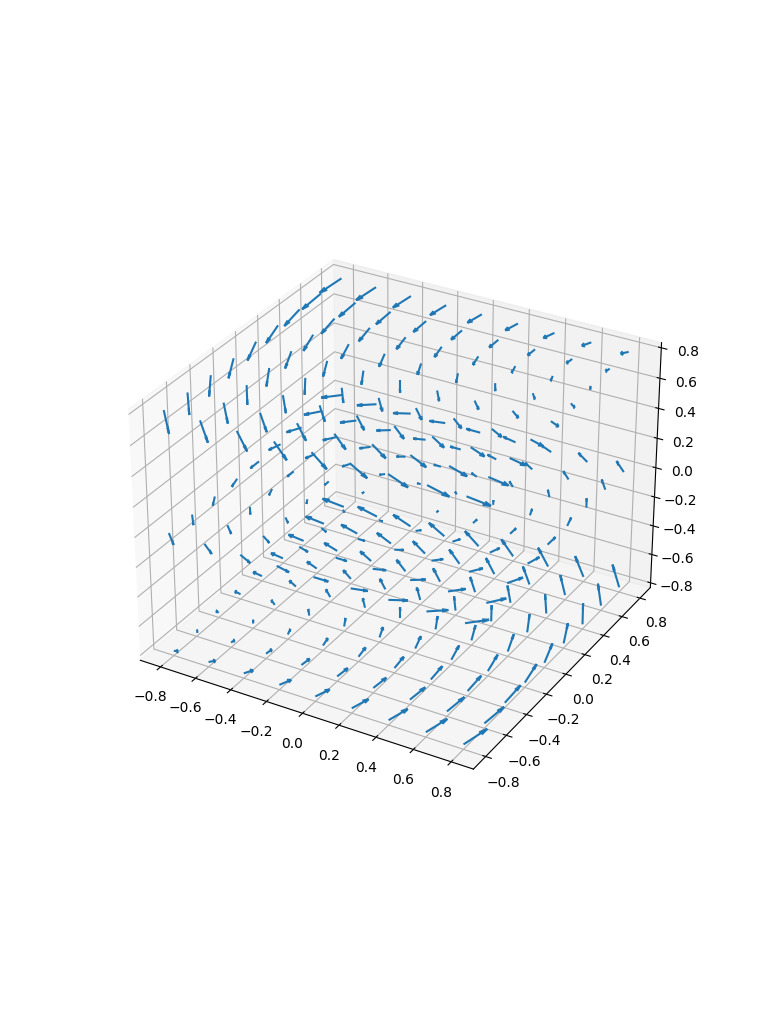
\includegraphics[width=\linewidth]{figures/wind4.png}
		\caption{}
		\label{eq:wind5}
	\end{subfigure}
	\begin{subfigure}{0.32\linewidth}
		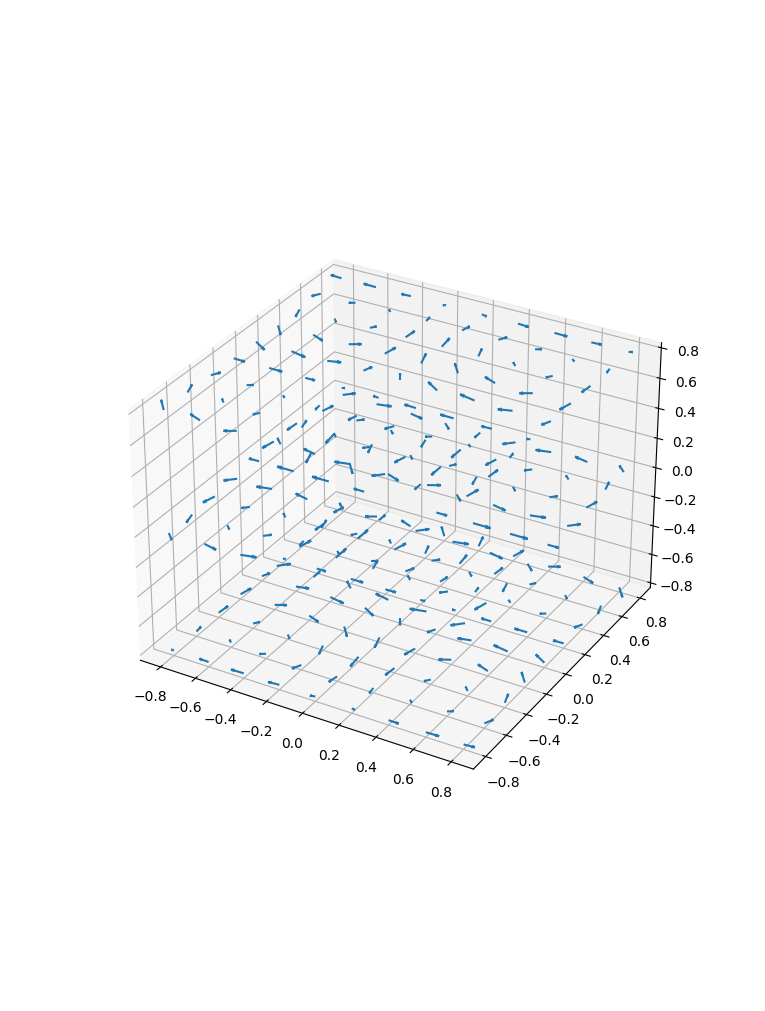
\includegraphics[width=\linewidth]{figures/wind2.png}
		\caption{}
		\label{fig:wind1}
	\end{subfigure}
	\begin{subfigure}{0.32\linewidth}
		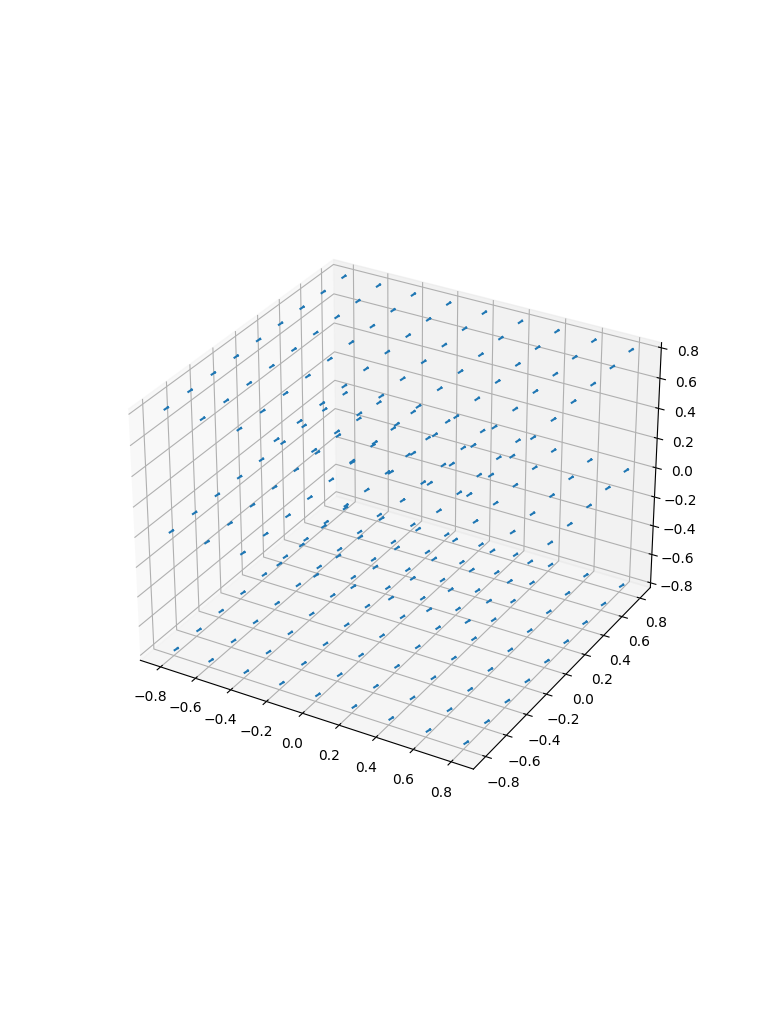
\includegraphics[width=\linewidth]{figures/wind3.png}
		\caption{}
		\label{fig:wind0}
	\end{subfigure}
	\caption{Visualization of three different wind fields. Vectors represent a force vector that impacts the drone in the matching position. (a)  is a random vector field made with a 3D function, (b) a predefined trigonometric vortex vector field and (c) with a random linear vector field.}
\end{figure}
The \emph{Wind Class} is an essential class in order to simulate a turbulent condition. Basically the class returns a 3 dimensional force vector $W$ based on the $x,y,z$ position of the drone. This force vector is then applied in the environment and pushes the drone in the matching direction. On initialization the wind is given a force bound $\omega_w [N]$ and a type. All vectors are being clipped to this amount of force in order to simulate wind fields of different strengths. In addition, the clipping method adds some Gaussian distributed randomness to each coordinate with the clipped value as mean and a standard deviation of $0.003$. \\
\newline
\emph{Type 0} simulates a random, constant wind field that applies the same random force vector at each position (\cref{eq:wind0}). The random coordinates $r_i$ are chosen with respect to a Gaussian distribution with the mean of $\frac{\omega_w}{2}$ and a standard deviation of $0.03$. As a consequence, the length of the force vector $|\overrightarrow{W}|$ is distributed with a mean of $0.866w$. A visualization of type 0 wind fields can be seen in \cref{fig:wind0}.
\begin{align} \label{eq:wind0}
	\overrightarrow{W} &= clip(\left(
	\begin{array}{c}
		r_0\\
		r_1\\
		r_2\\
	\end{array}
	\right))\\
	r_i &\sim \mathbb{N}(\frac{\omega_w}{2}, 0.03)\\
	\mathbb{E}|\overrightarrow{W}| &= \sqrt{3 \cdot \frac{\omega_w^2}{4}} \approx 0.866 \omega_w
\end{align}

\newpage

\emph{Type 1} is a trigonometric wind field with central vortex. A visualization can be seen in \cref{fig:wind1}.
\begin{align} \label{eq:wind1}
	\overrightarrow{W} = clip(\left(
	\begin{array}{c}
		\sin(\pi \cdot x) \cdot \cos(\pi \cdot y) \cdot \cos(\pi \cdot z)\\
		- \cos(\pi \cdot x) \cdot \sin(\pi \cdot y) \cdot \cos(\pi \cdot z)\\
		\sqrt{\frac{2}{3}} \cdot \cos(\pi \cdot x) \cdot \cos(
		\pi \cdot y) \cdot \sin(\pi \cdot z)\\
	\end{array}
	\right))
\end{align}
\newline

\emph{Type 2} is a wind field that is linear in each axis. Like seen in type 0 wind fields a random Gaussian distributed factor $r_i$ is used that indicate how steep each of the linear functions is.
\begin{align}
	\overrightarrow{W} &= clip(\left(
	\begin{array}{c}
		r_0 \cdot x\\
		r_1 \cdot y\\
		r_2 \cdot z\\
	\end{array}
	\right))\\
	r_i &\sim \mathbb{N}(\frac{\omega_w}{2}, 0.03)
\end{align}
\newline

\emph{Type 3} simulates a basic, random wind field with a central vortex. Therefore, it uses random signs.
\begin{align}
	\overrightarrow{W} &= clip(\left(
	\begin{array}{c}
		\pm y\\
		\pm x\\
		\pm z\\
	\end{array}
	\right))
\end{align}
\newline

\emph{Type 4} is a random wind field with a central vortex, that shows a little more complexity.
\begin{align}
	\overrightarrow{W} &= clip(\left(
	\begin{array}{c}
		x \pm y\\
		z \pm x\\
		y \pm z\\
	\end{array}
	\right))
\end{align}
\newline

\emph{Type 5} is a completely random wind field based on three random 3D functions $f, f', f'': \mathbb{R}^3 \to \mathbb{R}$. As a consequence, a lot of different, complex wind field can be created like seen in \cref{eq:wind5} that possesses different functions in each coordinate.\\

A \emph{3D function} can have a lot of different forms and should be described inductive. There are a base set of functions mapping from $\mathbb{R}^3 \to \mathbb{R}$ (\cref{eq:base}). In addition, there are two rules that inductively form the whole set of functions. If $g$ already is a 3DFunction then also $\sin(g), \cos(g), 2 \cdot x \cdot \sin(g), \sqrt{g}, e^g$ are 3DFunctions (\cref{eq:rule0}). If $g$ and $h$ are 3DFunctions then $g+h$ is also a 3Dfunction (\cref{eq:rule1}). Since there could be an endless regression, the induction is closed after only one step in order to avoid a stack overflow in implementation. 

\newpage
\begin{align}
	&\textbf{Base set:} \notag \\
	&F^0 = \{0, 1, x + y + z, x + y, x + z, y + z, 
	x \cdot y \cdot z, x \cdot y, x \cdot z, y \cdot z\} \label{eq:base}\\
	&\textbf{Rules:} \notag \\
	&\forall n < 2 \quad g \in F^n \land h \in F^n \rightarrow F^{n+1} = F^n \cup \{ 
	 g + h\} \label{eq:rule0}\\
	&\forall n < 2 \quad g \in F^n \rightarrow F^{n+1} = F^n \cup \{ \sin(g), \cos(g), 2 \cdot x \cdot \sin(g), \sqrt{g}, e^g\} \label{eq:rule1}
\end{align}
\newline
If no type is specified, then the wind field is of a chosen random type.
Since type 5 is the most complex type of wind field, the others might not be really needed, because similar wind fields like a vortex can still be approximated with the use of the 3D functions. However, it is still preferable to be able to choose a simple wind field at first before increasing complexity. In addition, there is the possibility to evaluate agents in different wind fields.

\subsection{Modes}\label{sec:modes}
Since the WindSingleAgentAviary class is meant as flexible class that more complex classes can inherit from, it has different modes that influence the position of the goal and the type of the wind (\cref{tab:mode}).
The use of modes is helpful in order to debug the environment end slowly increment the complexity of the RL problem.

\begin{table}[htp]
	\centering
	\caption{The different Modes of a WindSingleAgentAviary environment.}\label{tab:mode}
	\begin{tabular}{|c|c|c|c|}
		\hline
		Mode & Goal & Starting State & Wind\\
		\hline
		0 & $\overrightarrow{g} =\left(\begin{array}{c}
			0\\
			0\\
			0.5\\
		\end{array}
		\right)$ & $\overrightarrow{p_0} = \left(\begin{array}{c}
			0\\
			0\\
			0.5\\
		\end{array}
		\right)$ & no wind\\
		\hline
		1 & $\overrightarrow{g} = \left(\begin{array}{c}
			0\\
			0\\
			0.5\\
		\end{array}
		\right)$ & $\overrightarrow{p_0}\left(\begin{array}{c}
			0\\
			0\\
			z_{min}\\
		\end{array}
		\right)$ & no wind\\
		\hline
		2 & $\overrightarrow{g} \sim G_{HS}(R) $& $\overrightarrow{p_0}\left(\begin{array}{c}
			0\\
			0\\
			z_{min}\\
		\end{array}
		\right)$  & no wind\\
		\hline
		3 & $\overrightarrow{g} \sim G_{HS}(R) $& $\overrightarrow{p_0}\left(\begin{array}{c}
			0\\
			0\\
			z_{min}\\
		\end{array}
		\right)$  & specified type\\
		\hline
		%4 & $\overrightarrow{g} \sim G_{HS}(R) $& $\overrightarrow{p_0}\left(\begin{array}{c}
		%	0\\
		%	0\\
		%	z_{min}\\
		%\end{array}
		%\right)$  & random type\\
		%\hline
	\end{tabular}
	\label{tab:modes}
\end{table}

\newpage
\begin{algorithm}
	\caption{Evenly distributed Sampling from a half sphere $G_{HS}$}
	\label{alg:sample}
	\KwIn{radius $R$}
	\KwOut{goal $\overrightarrow{g} = \left(\begin{array}{c}
			g_x\\
			g_y\\
			g_z\\
		\end{array}
		\right)$ }
	
	\Repeat{$|\overrightarrow{\nu}| \leq R$}{
		$\overrightarrow{\nu} = \left(\begin{array}{c}
			\nu_x\\
			\nu_y\\
			\nu_z\\
		\end{array}
		\right) \qquad \nu_x, \nu_y \in [-R, R], \quad \nu_z \in [0,R]$
	}
	
	\Return $ \left( \begin{array}{c}
		0 \\
		0 \\
		0.5\\
	\end{array}\right) + \overrightarrow{\nu}$
	
\end{algorithm}
\emph{Mode 0} and \emph{Mode 1} are simple modes with a static goal $0.5 m$ over the ground and no wind, which only differ in the starting state distribution. In Mode 0 the drone is already in the goal and only has to stay there. In Mode 1 it starts on the ground and has to fly to the goal and hover there. Since the coordinate frame of the drone might not be on the lowest point, the drone starts at the height $z_{min}$.\\
\emph{Mode 2} evenly samples the goal vector from a half sphere that is shifted about $0.5$ in positive $z$ direction. 
This random point sampling in a half sphere is implemented with \cref{alg:sample}. It samples a random vector from inside a cupoid with the side lengths of $2 \cdot R, 2 \cdot R, R$ until it is inside the defined half sphere. As a consequence, the vector in evenly distributed. At first, this algorithm seems pretty inefficient, because in theory the break condition of the loop might never be violated. Hower, since the probability of $|\overrightarrow{\nu}| > R$ is small (\cref{eq:prob}),
the expected amount of loops is approximately $1.738$ (\cref{eq:expn}).
\begin{align}
	P(|\overrightarrow{\nu}| > r) &= 1 - \frac{V_{HS}}{V_Q} = 1 - \frac{\frac{2}{3} \cdot \pi R^3}{4 \cdot R^3} = 1 - \frac{1}{6} \cdot \pi \approx 0.476 \label{eq:prob}\\
	&\frac{d}{dq} \sum_{i=0}^{\infty} q^i = \frac{d}{dq} \frac{1}{1 - q} \qquad \forall |q| < 1\nonumber\\
	&\leftrightarrow \sum_{i=0}^{\infty} i \cdot q^{i-1} = \frac{1}{(1-q)^2} \qquad \forall |q| < 1 \nonumber\\
	&\leftrightarrow \sum_{i=0}^{\infty} i \cdot q = \frac{q}{(1 - q)^2} \qquad \forall |q| < 1 \\
	\mathbb{E}(n) &= \sum_{i = 0}^{\infty} (1 - \frac{1}{6} \cdot \pi)^i \cdot i  = \frac{ (1 - \frac{1}{6} \cdot \pi)}{(1 -  (1 - \frac{1}{6} \cdot \pi))^2}\approx 1.738 \label{eq:expn}
\end{align}
\emph{Mode 3} samples the goal with \cref{alg:sample}, but also implements a wind field. The type of the wind field is either given in initialization or random. Also the force bound is given in initialization. 
\newpage

\subsection{Observation Space \& State Space}
The state space $S$ defines the state vector of the drone in the environment and possesses a dimensionality of $23$. This state is only used inside the environment and consists of the current position $x_p, y_p, z_p$ in each axis, the roll, pitch and yaw angles $\Theta_p, \phi_p, \psi_p$ as well as represented as quaternion $q$, the velocities $\dot{x_p}, \dot{y_p}, \dot{z_p}$, the angular velocities $dot{\Theta_p}, \dot{\phi_p}, \dot{\psi_p}$, the goal position $x_g, y_g, z_g$ and the last clipped action $a_t$. With the use of this drone state space the observations are calculated.\\
\newline
The observation space $\daleth$ is a subset of the state space $S$ with the dimensionality of 15. The observation space is implemented as a \emph{spaces box} of type \emph{float32} which are mainly ranged within $[-1, 1]$ with the exception of the z coordinate of the position $z_p$ and goal $z_g$. Because there is floor defined as a plain at the height of $0$, which inherits a collision body, the drone is not able to reach a negative z coordinate. As a consequence, these are ranged to $[0,1]$.
\newline
\begin{align}
	\daleth_t &= (p_x,p_y,p_z, \Theta_p, \phi_p, \psi_p, \dot{p_x}, \dot{p_y}, \dot{p_z}, \dot{\Theta_p}, \dot{\phi_p}, \dot{\psi_p}, g_x, g_y, g_z) \label{eq:obs}
\end{align}
\newline
Each observation $\sigma_t$ consists of the current position $x_p, y_p, z_p$ in each axis, the roll, pitch and yaw angles $\Theta_p, \phi_p, \psi_p$, the velocities $\dot{x_p}, \dot{y_p}, \dot{z_p}$, the angular velocities $\dot{\Theta_p}, \dot{\phi_p}, \dot{\psi_p}$ and the goal position $g_x, g_y, g_z$ (\cref{eq:obs}). These observations are given to the NN in order to approximate the optimal action $a$ that satisfies the defined RL problem.\\
\newline
Like previously mentioned, all observations are ranged in order to prohibit inputs of different magnitude that could disrupt the learning process. This is done with the use of the method \emph{\_clipAndNormalizeState} which gets the current state $s_t$ and normalizes it to the defined range (\cref{eq:clipnorm}). First, it clips it to predefined values $v$ and then normalizes it by dividing with the matching predefined value $v_i, i\in[0,11]$. If wanted, a warning can be printed each time a state parameter has to be clipped. By clipping x and y to a value in $[-20,20]$ there is a predefined limit of maximal distance, in which there is a reasonable option to learn robust flight. Analogue the z component is clipped to $[-10,10]$, roll and pitch to $[-\pi, \pi]$, the translation velocities to $[-3, 3]$ in $x, y$ and to $[-2,2]$ in $z$ direction. 
\newline
\begin{align}
	\daleth_t \leftarrow clip(s_t) / v \label{eq:clipnorm}
\end{align}
\newline

\newpage

\subsection{Action Space}
The WindSingleAgentAviary Environment possesses three different type of action spaces, that are processed in different ways to the \emph{rpm (rotation per minute)} of the four motors (\cref{tab:act}). Nevertheless, all action types are continuous and are ranged in $[-1, 1]$.\\
\newline
\emph{one\_d\_rpm} is a one dimensional action space. The chosen action $a$ is processed to range of $0.05$ about the \emph{hover\_rpm} to a 4-tupel of rpms. The hover\_rpm is defined as the rpm that corresponds to hovering (\cref{sec:hover}). The 4-tupel is then forwarded to the motors. As a consequence of this limitation, the drone can only perform hovering, rising and falling movements and can not influence its $x,y$ position or $\Theta, \phi, \psi$. Also, the translational speed $v_z$ is limited by the size of $0.05$.\\
\newline
\emph{rpm} is a 4 dimensional action space. The actions are processed within a range of $0.05$ about the hover\_rpm to a 4-tupel of rpms. The drone is not limited in any dimensionality, but the task increases in complexity. Due to \cref{form:quad}, \cref{form:quad2}, \cref{form:quad3}, \cref{form:quad4} even a small difference in rpms can lead to an unstable flight or even a crash, because the roll or pitch angle is too high. Also, all translational and rotational speeds are limited by the size of $0.05$. Because of the higher complexity, it is expected, that the training takes noticeable more time.\\
\newline
\emph{vel} is a top level, 4-dimensional action space. The action consists of a velocity vector $v = (a_0, a_1, a_2)$ and its size $a_3$.  Since it is a top level action space, the actions are not corresponding directly to the rpms, but a pid controller (\cref{sec:pid}) is used in order to control the rpms. The basic pid controller is part of Gym Pybullet Drones \cite{panerati2021learning} and must be tuned for the used quadrocopter. It mainly receives the state $S$ of the drone, as well as the targeted velocity, which is calculated with the use of the actions. Therefore, $a_3$ is multiplied with speed limit of the drone in order to derange the action. Also, the velocity vector $\overrightarrow{v}$ is normalized to a length of $1$.\\
The drone is not limited in any dimensionality and the task is less complex than setting rpm directly. Stability of the flight is now mainly controlled by the pid controller, so it is bounded by the typical pid constraints in harsh environments and not adaptable.
\begin{table}
	\centering
	\caption{The different ActionTypes with the corresponding dimensionality of the action, its range and how it is processed.}\label{tab:act}
	\begin{tabular}{c|c|c|c}
		ActionType & dim & range & processing\\
		\hline
		\emph{one\_d\_rpm} & $|a| = 1$ & $a_i \in [-1, 1]$ & $rpm = (hover\_rpm \cdot (1 + 0.05 \cdot  a)) \cdot (1, 1, 1, 1)$ \\
		\emph{rpm} & $|a| = 4$ & $a_i \in [-1, 1]$ & $rpm =  hover\_rpm \cdot (1 + 0.05 \cdot  a)$ \\
		\emph{vel} & $|a| = 4$ & $a_i \in [-1,1]$ & $rpm = pid(S, vel= limit \cdot  |a_3| \cdot \frac{(a_0,a_1,a_2)}{|(a_0,a_1,a_2)|})$
	\end{tabular}
\end{table}


\newpage

\subsection{Reward Function}
\begin{figure}
	\centering
	\begin{subfigure}{0.32\linewidth}
		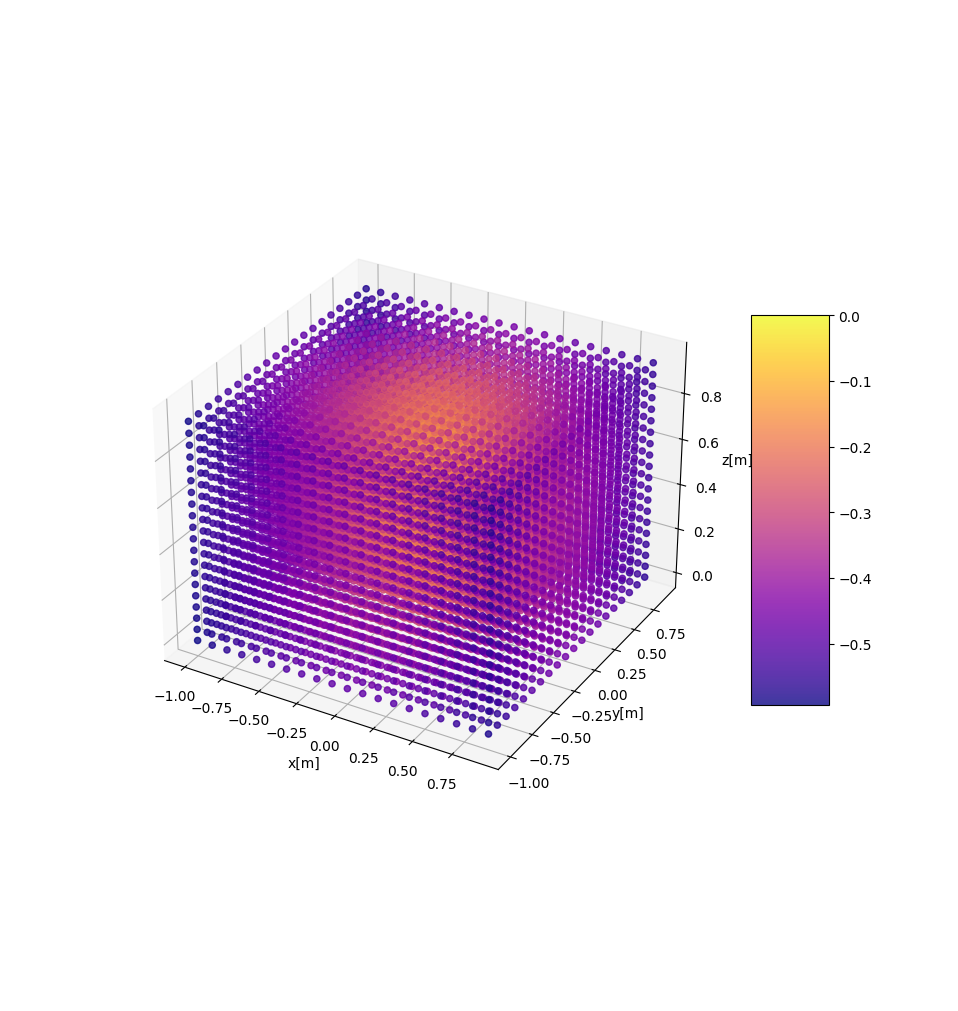
\includegraphics[width=\linewidth]{figures/rew3d.png}
		\caption{}
	\end{subfigure}
	\begin{subfigure}{0.32\linewidth}
		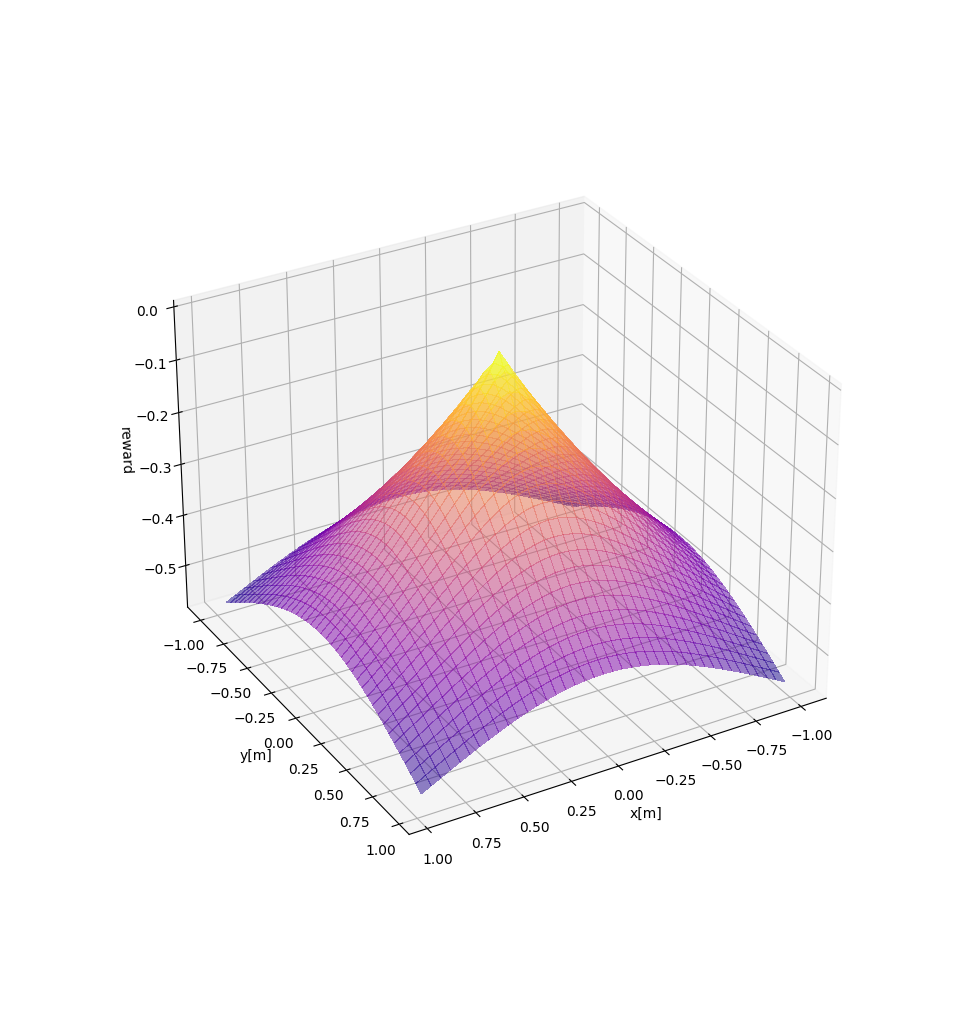
\includegraphics[width=\linewidth]{figures/rewXY.png}
		\caption{}
	\end{subfigure}
	\begin{subfigure}{0.32\linewidth}
		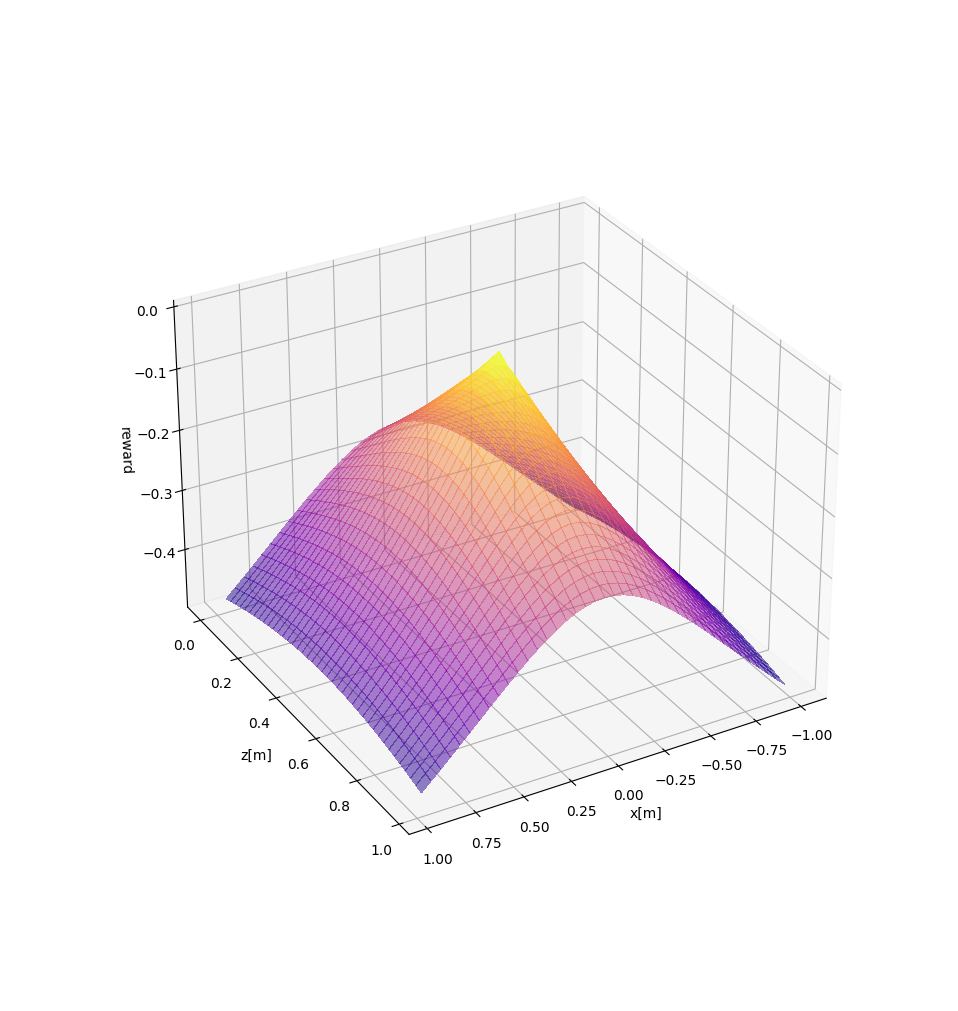
\includegraphics[width=\linewidth]{figures/rewXZ.png}
		\caption{}
	\end{subfigure}
	\caption{Visualization of the used reward function with the goal ($0,0,0.5$) and a color scale for different positions in space.}
	\label{fig:rewr}
\end{figure}
The reward mainly assesses how the agent learns and which action are benefitial in which state.
In this environment the reward consists of a classic reward function, mainly depending on the distance to the goal $dist_t$ (\cref{eq:rew}), and a set of constraints.\\
The reward function is an exponential function with a negative exponent. The factor $0.6$ defines the steepness of the function. \cref{fig:rewd} shows a plot of the reward function over a small field of distances up to $2m$.  Due to the main exponential part, the reward function is also bounded to the range $[-1, 0]$ with the gradient increasing close to a distance of $0$. This is helpful in order to get a precise behavior. At hughe distances the gradient is small, but this does not really matter that much because so hughe distances are not expected.
\begin{align}
	r_t = e^{-0.6 \cdot dist_t} - 1 &= e^{-0.6 \cdot |\overrightarrow{g} - \overrightarrow{p_t}|} - 1 \label{eq:rew}\\
	\lim_{dist_t \to \infty} r_t &= -1\\
	\lim_{dist_t \to 0+} r_t &= 0
\end{align}
As a consequence, the reward function only depends on the current relative position to the goal. The action with the highest reward is the action that concurrs with the optimal velocity vector towards the goal while still guaranteeing a safe flight. \cref{fig:rewr} also shows this relation with the standard goal $g=(0, 0, 0.5)$ of mode 0 and mode 1. The reward towards a fixed goal is point semetric with the global maximum when $dist_t = 0$.

\newpage

\begin{figure}
	\centering
	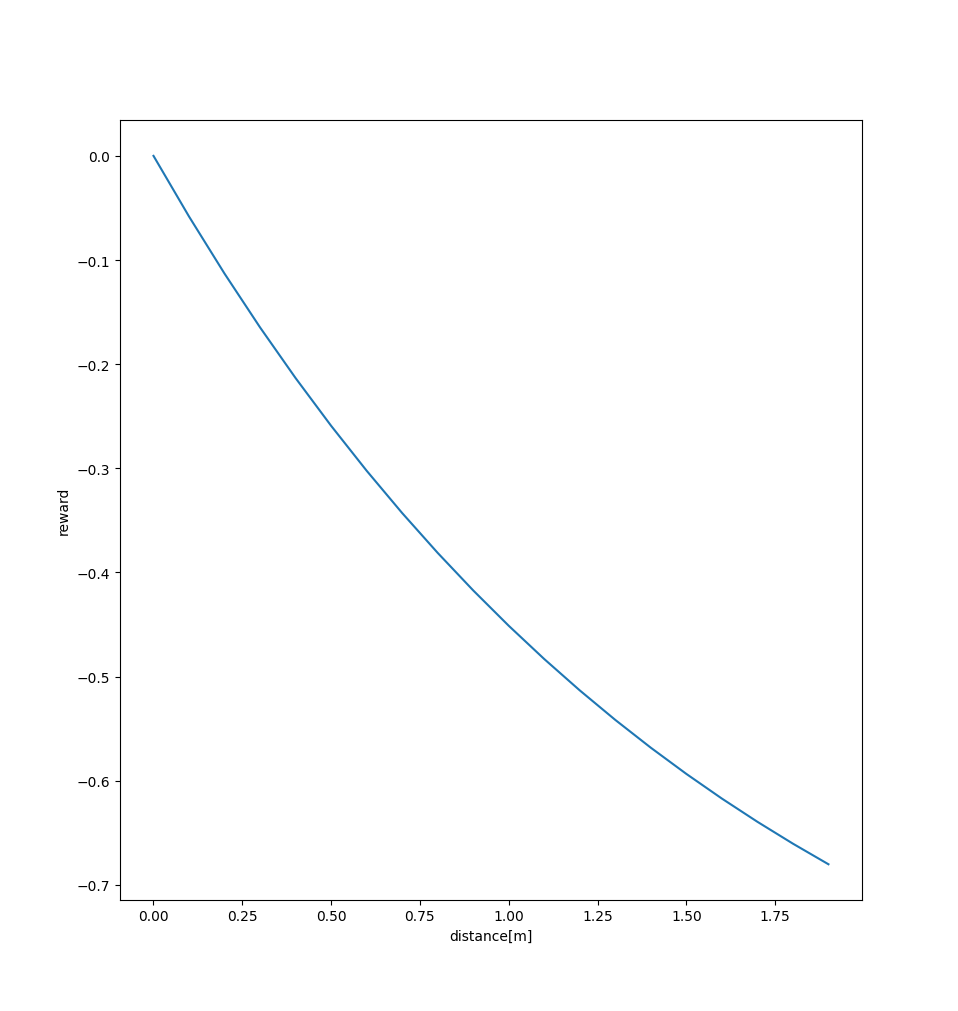
\includegraphics[width= 0.5\linewidth]{figures/reward.png}
	\caption{Visualization of the reward functions over the total distance[m]}
	\label{fig:rewd}
\end{figure}

\subsection{Constraints}
Besides, the reward function is also unfluenced by a set of constraints, which are logical rules that define a safe flight. If one of the rules is broken, the episode is ended by returning a done $d$ value that is true. In addition, there is a punishement reward of $-200$ that is added to the classic reward function.\\
This constraints can be benefitial for training time, because the episodes are ended early. Also, unsafe flight is highly unattractive for the agent because of the punishement reward. 
\begin{align}
	p_{z} \leq z_{min} \land \frac{t_s}{f_s} \geq 0.1 s \to r_t &= e^{-0.6 \cdot |goal - pos|} - 1 -200 \land d = True \label{con:1}\\
	\Theta_p > 1 \lor \phi_p > 1 \to r_t &= e^{-0.6 \cdot |goal - pos|} - 1 -200 \land d = True \label{con:2}
\end{align}
The first constraint (\cref{con:1}) is checking if the UAV crashed. Therfore, it compares the height of the coordinate frame with the starting height $z_{min}$ and checks that already some time has passed. This is needed, because otherwise the constraint would fire directly when starting. If this rule fires, $200$ is subtracted from the reward as punishement and the episode is ended. 
As a consequence the agent learns to avoid crashing and to start fast.\\
The second constraint (\cref{con:2}) is checking the roll and the pitch angle. If one of these angles is bigger than $\approx 57,296^{\circ}$ the rule fires and leads to a terminal state and a punishement. As a consequence the agent learns stable flight and avoids this undesired states. The roll and pitch angle should be kept as close as possible to zero. However, in order to change the $x,y$ coordinates a roll and pitch angle is needed. Also, this might be benefitial countering wind.

\newpage

\subsection{Optimal Rewards}
Based on the modes (\cref{sec:modes}) different optimal rewards (\cref{eq:rew}) can be defined, that are helpful in order to determine how good the learned decision making is.\\
\emph{Mode 0} has an optimal reward of $r_{opt} = 0$, which is basically just giving the action $0$ to all motors. This leads to hovering and staying in the goal.
\emph{Mode 1} is due to its fixed goal position $g$ rather easy to define:
\begin{align}
r_{opt} &= \sum_{t=0}^{f_c \cdot T}  r_{opt_t} \label{eq:oprew}\\
d_0 &= 0.5\\
dist_{t+1} &= dist_t - |\overrightarrow{v_{opt}}| \cdot \frac{1}{f_c} \label{eq:dt1}%\\
%r_{t} &= e^{-0.6 \cdot (d_{t+1} )} - 1 \label{eq:rew2}
\end{align}
The distance at start $d_0$ is always 0.5. An optimal decision of the agent corresponds to an optimal velocity vector $v_{opt}$ that minimizes the distance to the goal with the given bounds of the maximum speed at the $\alpha$ of the action processing. The reward (\cref{eq:rew}) can then be used for every control step and summed up to the total optimal reward $r_{opt}$ (\cref{eq:oprew}).\\
Since every mode apart from mode 0 and mode 1 does not possess a fixed goal position, only an expected optimal reward $\mathbb{E}(R_{opt})$ can be defined. Therefore, an expected starting distance $\mathbb{E}(d_0)$ to a goal that is equally distributed in a half sphere:
\begin{align}
	\mathbb{E}(d_0) &= \sqrt{\mathbb{E}(d_x)^2 + \mathbb{E}(d_y)^2 + \mathbb{E}(d_z)^2}  = \mathbb{E}(d_z) \\
	\mathbb{E}(d_x) &= \mathbb{E}(d_y) = 0\\
	\mathbb{E}(d_z) &= 0.5 + \mathbb{E}(z^*) = 0.5 + P(z) \cdot \int \int \int  z dx dy dz \nonumber \\
	&= 0.5 + \frac{1}{V} \int_{0}^{2 \cdot \pi} d \phi \int_{0}^{\frac{\pi}{2}} \sin(\Theta) d\Theta \int_{0}^{R} r^2 r \cos(\Theta)  dr  \nonumber \\
	&= 0.5 + \frac{\frac{\pi}{4} R^4}{\frac{2}{3} \pi R^3} = 0.5 + \frac{3}{8} R
\end{align}
The expected distance in each axis $\mathbb{E}(d_0)$ depends linear on the chosen maximum radius $R$. The expected distance in $x$ and $y$ direction is equal to zero due to the symmetrie of the half sphere.\\
Also mode 3 possess a wind class that tries to disrupt the agent. Since there are random wind fields and the corresponding force is not normally distributed, the optimal reward can just be estimated downwards. Therefore, the used maximum wind force $\omega_w$ is used in order to approximate the maximum of disruptive distance and use it in order to update \cref{eq:dt1}.
\begin{align}
	dist_{t+1} &= dist_t - | v_{opt} | \cdot \frac{1}{f_c} + \frac{\omega_w}{m} \cdot \frac{1}{f_c}
\end{align}
\newpage

%\subsection{WindSingleAgentPathfollowingAviary Environment Class}


\newpage

%%%%%%%%%%%%%%%%%%%%%%%%%%%%%%%%%%%%%%%%%%%%%
\section{Scripts \& Evaluation Tools} \label{sec:scripts}
In order to learn a policy $\pi$ based on the implemented environment a learning script was implemented that offers parsing different arguments $\xi$. These arguments define the learning process and different environment arguments $\tilde{\lambda}$, that are used on initialization of the WindSingleAgentEnvironment class.
Also, the evaluation script offers a similar script with similar arguments $\xi$ in order to evaluate the policy $\pi$.
Therfore, it uses two different evaluation tools and the gym-pybullet-drones logger. 

%\subsection{TestInstall Script}

\subsection{Learning Script}
The learning script (\cref{alg:learn}) receives a set of parsed arguments $\xi$ (\cref{tab:learningparse}) and checks them on contradictions. If a predefined contradiction is found a \emph{ParsingError} is raised stating the contradicting parsed arguments with a message.
Then, the training environment $\epsilon_t$ is created with the parsed environment args $\tilde{\lambda} \subset \xi$ and the policy is defined based on the parsed algorithm. The policy mocel $\pi$ is then either created or loaded from a specified file. Next, a evaluation environment $\epsilon_e$ is created with the same arguments and the evaluation callbacks are defined. Then depending on the parsed curriculum parameter $\zeta$ the policy is either trained commonly or with a curriculum method (\cref{alg:curri}).
At last, the policy model $\pi$ is safed with the parsed name.

\begin{longtable}{|c|c|c|c|c|}
	\caption{Overview of the Arguments $\xi$ parsed to the Learning Script}\label{tab:learningparse}\\
	
	\hline
	Name & Symbol & Type & Default & Explaination\\
	\hline
	%\toprule
	\endfirsthead
	\caption[]{Overview of the Arguments $\xi$ parsed to the Learning Script}
	\endhead
	
	--cpu &  $\eta$ & Integer & $1$ & Amount of parallel\\
	& & & &  training environments\\
	\hline
	--drone & & DroneModel & $Dronemodel.HB$ & The drone model\\
	\hline
	--steps & $t_{total}$ & Float & $1e7$ & Training steps \\
	\hline
	--mode & & Integer & $0$ & Environment mode\\
	\hline
	--load & $\iota$ & Boolean & $false$ & Load an existing policy\\
	\hline
	--total\_force & $\omega[N]$ & Float &  $0.0$& The upper force bound\\
	\hline
	--radius & $R[m]$ & Float & $0.0$ & The default radius\\
	\hline
	--debug\_env & & Boolean & $false$ & Enables debug print \\
	& & & & statements in the \\
	& & & & environment\\
	\hline
	--episode\_len & $T[s]$ & Integer & $5$ & Amount of seconds of \\
	& & & & each episode\\
	\hline
	--act & & ActionType & $ActionType.RPM$ & The type of action \\
	& & & & of the NN\\
	\hline
	--name & & String & $"results$ & The name of the model \\
	& & & $/success$ & after training\\
	& & & $\_model.zip"$ & \\
	\hline
	--curriculum & $\zeta$ & Boolean & $false$ & Use curriculum learning\\
	\hline
	--algo & & String & $"ppo"$ & The used algorithm\\
	\hline
\end{longtable}

\newpage

\begin{algorithm}
	\caption{Learning Script}
	\label{alg:learn}
	\KwIn{parsed arguments $\xi$}
	
	Check the parsed arguments $\xi$ on contradiction and raise ParsingError if needed
	
	Create training environment $\epsilon_t$ with the parsed environment args $\tilde{\lambda} \subset \xi$
	
	Define relevant attributes for the policy network
	
	\If{parsed load parameter $\iota \in \xi$}{
		Load policy model $\pi$ with matching algorithm
	}
	\Else{
		Create policy model $\pi$ with matching algorithm
	}
	
	Create evaluation environment $\epsilon_e$ with the parsed environment args $\lambda \subset \xi$
	
	Define evaluation callbacks
	
	\If{parsed curriculum parameter $\zeta \in \xi$ is parsed as false}{
		Learn the model with the parsed amount of time steps
	}
	\Else{
		Learn the model with the curriculum method (\cref{alg:curri})
	}
	
	Save the model $\pi$ with the parsed preferred name
	
	
\end{algorithm}

\subsubsection{Linear Curriculum Learning}
\emph{Linear Curriculum Learning (LCL)} is a method that changes environment parameters during training process. In contrast, the classic approach uses the parsed algorithm in order to optimize the policy on a firm environment. LCL is a simple adaption that changes an environment parameter after a specified amount of steps. In this case, the radius parameter $R$ of the environment is adjusted. In Theory, the learning starts with a rather simple approach with a fixed goal and then steadily increases the difficulty of the RL problem, which may benefit training performance.\\
The LCL algorithm (\cref{alg:curri}) receives the total steps within a unchanged environment $t_total$, a set of environment args $\tilde{\lambda}$, the policy model $\pi$, the amount of parallel environments $\eta$ and the specified name of the model.
Then the maximum radius $R_{max}$ is saved from $\tilde{\lambda}$ and the current radius $R$ is initialized with a value of $0$.
Until the current radius is bigger or equal to the maximum radius, the radius in $\tilde{\lambda}$ is set to the current radius. Also, the training environment $\epsilon_t$ with the new arguments is initialized and set, the evaluation environment $\epsilon_e$ is initialized and evaluation callbacks are defined. Then, the policy model is learned in a common way with $t_total$ steps. Due to the evaluation callbacks it may be that the learning starts earlier if the policy outperforms a defined performance threshold. At last, the policy is saved, the best policy $\pi_{best}$ is renamed and the current radius $R$ is linear increased.

\newpage

\begin{algorithm}
	\caption{Linear Curriculum Learning Algorithm}
	\label{alg:curri}
	\KwIn{total steps $t_{total}$,  set of environment args $\tilde{\lambda}$, model $\pi$, number of parallel environments $\eta$, name}
	
	Get radius $R_{max}$ from $\tilde{\lambda}$
	
	$R = 0.0$
	
	\While{$R \leq R_{max}$}{
		Change radius in $\tilde{\lambda}$ ro R
		
		Initialize training environment $\epsilon_t$ with $\tilde{\lambda}, \eta$ as parameters
		
		Set $\epsilon_t$
		
		Initialize evaluation environment $\epsilon_e$ with $\tilde{\lambda}, \eta$ as parameters
		
		Define evaluation callback
		
		Learn the model $\pi$ with the amount of steps $t_{total}$
		
		Save $\pi$ and rename best policy $\pi_{best}$
		
		$R = R + 0.2$
	}
\end{algorithm}

\subsection{Evaluation Script}
The evaluation script (\cref{alg:eval}) is structured similar to the algorithm script and also receives a set of
parsed arguments $\xi$ (\cref{tab:evalparse}). First, it checks $\xi$ on contradiction and raises a ParsingError if needed. Then, the evaluation environment $\epsilon_e$ is created with the parsed set of environment args $\tilde{\lambda}$ and the policy model $\pi$ is loaded. The \emph{EvalWriter} class (\cref{sec:evalw}) is then instatiated and used for evaluation.\\
If the gui parameter $\tilde{\rho}$ is parsed a single episode is visualized with the pybullet gui. 
Therefore, a test environment $\epsilon_t$, a logger and a pathplotter class is instantiated.
At the start, the environment is reset and returns an initial observation $\daleth_0$. In order to sync the simulation time to the real word time the current real time $t^*$ is safed.
Until the episode is over a fixed amount of commands are executed:\\
\newline
First $\pi$ is used in order to decide the action $a$. The action is then given to $\epsilon_t$ and a step is executed that returns a reward $r_t$, a done value $d$ and an info.
Then, the current pose vector $\overrightarrow{p_t}$ is added to the pathplotter class and the current drone state $s_t$ is logged with the logger. At last, the simulation time $t_{sim}$ is synced to the real time $t^*$.\\
\newline
After this visualization the environment is closed, the plotted path and the logs are shown.

\newpage

\begin{longtable}{|c|c|c|c|c|}
	\caption{Overview of the Arguments $\xi$ parsed to the Evaluation Script}\label{tab:evalparse}\\
	
	\hline
	Name & Symbol & Type & Default & Explaination\\
	\hline
	%\toprule
	\endfirsthead
	\caption[]{Overview of the Arguments $\xi$ parsed to the Evaluation Script}
	\endhead
	
	--drone & & DroneModel & $Dronemodel.HB$ & The drone model\\
	\hline
	--episodes &  & Float & $100$ & Evaluation Episodes \\
	\hline
	--mode & & Integer & $0$ & Environment mode\\
	\hline
	--total\_force & $\omega[N]$ & Float &  $0.0$& The upper force bound\\
	\hline
	--radius & $R[m]$ & Float & $0.0$ & The default radius of\\
	& & & &  the goal sphere\\
	\hline
	--debug\_env & & Boolean & $false$ & Enables debug print \\
	& & & & statements in the \\
	& & & & environment\\
	\hline
	--episode\_len & $T[s]$ & Integer & $5$ & Amount of seconds of \\
	& & & & each episode\\
	\hline
	--init & $p_0$ & List[Float] & $none$ & Starting state\\
	\hline
	--gui & $\tilde{\rho} $& Boolean & $true$ & Show gui\\
	\hline
	--act & & ActionType & $ActionType.RPM$ & The type of action \\
	& & & & of the NN\\
	\hline
	--name & & String & $"results$ & The name of the model \\
	& & & $/success$ & after training\\
	& & & $\_model.zip"$ & \\
	\hline
	--algo & & String & $"ppo"$ & The used algorithm\\
	\hline
\end{longtable}

\begin{algorithm}
	\caption{Evaluation Script}
	\label{alg:eval}
	\KwIn{parsed arguments $\xi$}
	Check the parsed arguments $\xi$ on contradiction and raise ParsingError if needed
	
	Create evaluation environment $\epsilon_e$ with the parsed environment args $\tilde{\lambda} \subset \xi$
	
	Load the policy model $\pi$
	
	Instantiate an EvalWriter and evaluate the model $\pi$
	
	\If{parsed gui parameter $\tilde{\rho} \in \xi$}{
		Instantiate a test environment $\epsilon_t$, logger and a pathplotter
		
		Reset environment and safe an observation $\daleth_0$
		
		Safe current real time $t^*$
		
		\Repeat{episode is done}{
		Get action $a$ from $\pi$ based on $\daleth_t$
		
		Step $\epsilon_t$ and receive an observation $\daleth_t$, reward $r_t$, a done value $d$ and a info
		
		Add current pose $\overrightarrow{p_t}$ to pathplotter and log state $s_t$
		
		Sync simulation time $t_{sim}$ to the real time $t^*$}
		Close test environment, show the plotted path and logs
	}


\end{algorithm}

\newpage

\newpage

%%%%%%%%%%%%%%%%%%%%%%%%%%%%%%%%%%%%%%%%%%%%%%
\subsection{Evaluation Tools} \label{sec:tools}
In order to evaluate the policies and visualize the flight path, the \emph{EvalWriter} and the \emph{PathPlotter} class were implemented.
The EvalWriter class aims at providing a static metric that emphasises how good a chosen policy $\pi$ is. Therefore, it evaluates different classic RL metrics like the average accumulated reward and also some basic control theory metrics like overshoot (\cref{tab:evalmetric}).
The PathPlotter class aims at visualizing a single episode in a 3D plot.

\subsubsection{EvalWriter Class} \label{sec:evalw}
\begin{table}
	\centering
	\caption{The evaluation metric.}\label{tab:evalmetric}
	\begin{tabular}{c|c|c}
		Name & Form & Explanation\\
		\hline
		rate & $x \%$ & percentage of succeeding episodes\\
		time rate $\beth$ & $x\%$ & percentage of time in goal sphere\\
		settled rate & $x\%$ & percentage of settled episodes\\
		dist($\frac{T}{2}$) & $(x \pm y) m $& average distance half way through episode\\
		dist($T$) &  $(x \pm y) m $ & average distance at the end of the episode\\
		overshoot & $(x \pm y) m $ & average overshoot\\
		reward & $x \pm y $ & average accumulated episode reward
	\end{tabular}
\end{table}

The EvalWriter class is intialized with a name, a number of evaluation steps $\gimel$, the path to the xlsx file it writes to, the environment $\epsilon$, the episode length  $T$ and the threshold $\Omega[m]$ that defines a sphere around the goal. If the drone is inside this sphere and the distance is lower than $\Omega$ it counts a beeing in the goal. In theory this parameter could be fixed to 0, but it is easier to allow a minimum distance in order to compare the policies better.The EvalWriter has  an update function (\cref{alg:upd}), that is used in order get the new distances from $\epsilon$ and update the metric parameters and is used in the evaluation algorithm (\cref{alg:evalwriter}). Then, the data can be visualized with the \emph{write} method.

\begin{algorithm}
	\caption{Update Algorithm of EvalWriter}
	\label{alg:upd}
	Get current $dist$ and $t_{sim}$ from environment $\epsilon$ and save it
	
	\If{$e = 1$}{
		Add pose of the drone from $\epsilon$ to pathplotter
		}
		
	\If{$t_{sim} = \frac{T}{2}$}{
		Save current $dist$ to matching set of distances
		}
		
	\If{$t_{sim} = T$}{
		Save current $dist$ to matching set of distances
	}
	
	\If{episode already reached goal and overshoot}{
		Save current $dist$ to overshoot set
	}
	
	Check if the episode succeded in this time step
\end{algorithm}

\newpage

\begin{algorithm}
	\caption{Evaluation Algorithm of EvalWriter}
	\label{alg:evalwriter}
	\KwIn{policy $\pi$}
	\KwOut{tupel ($\mu_r, \sigma_r$)}
	
	Get mean reward $\mu_r$ and the std of the reward $\sigma_r$ from $evaluate\_policy (\pi , \epsilon, e)$
	
	reset $\epsilon$ and receive $\daleth_t$
	
	\For{$j=0 \to \gimel$}{
		\Repeat{$done$}{
			Get action $a$ from $\pi$ with input $\daleth_t$
			
			Step $\epsilon$ and get the new observation $\daleth_t$, reward $r_t$, a done signal $d$  and an info
			
			Update EvalWriter
			
			\If{$d$}{
				Reset $\epsilon$
				}
		}
		\If{not $j = \gimel$}{
			Use Housekeeping of the EvalWriter class
			}
	}
	Close EvalWriter and $\epsilon$.
	
	\Return ($\mu_r, \sigma_r$)
	
\end{algorithm} 

\subsubsection{PathPlotter Class}
The PathPlotter class is a basic class that visualizes the path taken by drone under a policy $\pi$. 
It is mostly used in the EvalWriter class when only a single episode is evaluated, but also can be used seperatly.
It mainly helps understanding the current decision making of a policy. On fixed goal modes it literaly sums up the complete performance in one plot.\\
 It is initiliaized with a set of goals $\overrightarrow{g}$. With the use of the \emph{addPose} method the position of the drone at different time steps can be added. After the episode, the drone path can be visualized with a \emph{Matplotlib 3D plot} by using the \emph{show} method, which creates plots like %\cref{fig:}.
